\documentclass[11pt,a4paper]{article}

\usepackage{graphicx}

% ---- Idioma y tipografía
\usepackage[spanish]{babel}
\usepackage[T1]{fontenc}
\usepackage[utf8]{inputenc}  % (si usas XeLaTeX/LuaLaTeX, elimínala)
\usepackage{lmodern}
\usepackage{microtype}

% ---- Márgenes y diseño
\usepackage[a4paper,margin=2.2cm]{geometry}
\usepackage{parskip}

% ---- Enlaces
\usepackage[hidelinks]{hyperref}
\usepackage{bookmark}

% ---- Cabeceras y pies
\usepackage{fancyhdr}
\pagestyle{fancy}
\fancyhf{}
\renewcommand{\headrulewidth}{0.4pt}
\cfoot{\thepage}

% ---- Listas y símbolos
\usepackage{enumitem}
\setlist{itemsep=0.25em, topsep=0.3em}

% ---- Iconos y color
\usepackage{fontawesome5}
\usepackage{xcolor}
\usepackage[most]{tcolorbox}
\tcbuselibrary{breakable,skins}

% ---- Colores propios
\definecolor{uniPrimary}{HTML}{0A7AC3}
\definecolor{uniSoft}{HTML}{E9F4FB}
\definecolor{uniAccent}{HTML}{F5B700}
\definecolor{uniOK}{HTML}{2E7D32}
\definecolor{uniWarn}{HTML}{C62828}

% ---- Metadatos reutilizables
\newcommand{\asignatura}{MULTIMEDIA}
\newcommand{\tema}{TEMA 2 — Conceptos básicos sobre la compresión de datos}
\newcommand{\clase}{Clase 2}
\newcommand{\fecha}{\today}

\usepackage{booktabs} % para tablas más bonitas
\usepackage{siunitx}  % para alinear números y usar unidades correctamente
\usepackage{amsmath}  % para fórmulas matemáticas

% ---- Cabecera con metadatos
\lhead{\textsc{\asignatura}}
\rhead{\textbf{\tema}}

% ---- Estética de secciones
\usepackage{titlesec}
\titleformat{\section}{\Large\bfseries\color{uniPrimary}}{\thesection}{0.5em}{}
\titleformat{\subsection}{\large\bfseries}{\thesubsection}{0.5em}{}
\titleformat{\subsubsection}{\bfseries}{\thesubsubsection}{0.5em}{}

% ---- Cajas útiles
\newtcolorbox{ObjetivosBox}{
	title={\faBullseye\; Índice},
	colback=uniSoft,
	colframe=uniPrimary,
	enhanced, breakable,
	left=8pt,right=8pt,top=8pt,bottom=8pt,
	boxrule=0.8pt,
	fonttitle=\bfseries
}

\newtcolorbox{DefBox}{
	title={\faBook\; Definición},
	colback=white,
	colframe=uniAccent,
	enhanced, breakable,
	left=8pt,right=8pt,top=8pt,bottom=8pt,
	boxrule=0.8pt,
	fonttitle=\bfseries
}

\newtcolorbox{NotaBox}{
	title={\faStickyNote\; Nota},
	colback=white,
	colframe=uniPrimary,
	enhanced, breakable,
	left=8pt,right=8pt,top=8pt,bottom=8pt,
	boxrule=0.8pt,
	fonttitle=\bfseries
}

\newtcolorbox{RecordatorioBox}{
	title={\faBell\; Recordatorio},
	colback=uniAccent!15,
	colframe=uniAccent,
	enhanced, breakable,
	left=8pt,right=8pt,top=8pt,bottom=8pt,
	boxrule=0.8pt,
	fonttitle=\bfseries
}

\newtcolorbox{ChecklistBox}{
	title={\faTasks\; Tareas / Checklist},
	colback=white,
	colframe=uniPrimary,
	enhanced, breakable,
	left=8pt,right=8pt,top=8pt,bottom=8pt,
	boxrule=0.8pt,
	fonttitle=\bfseries
}

\newtcolorbox{ResumenBox}{
	title={\faHighlighter\; Resumen rápido (5 líneas)},
	colback=uniSoft,
	colframe=uniPrimary,
	enhanced, breakable,
	left=8pt,right=8pt,top=8pt,bottom=8pt,
	boxrule=0.8pt,
	fonttitle=\bfseries
}

\newtcolorbox{VocabBox}{
	title={\faLanguage\; Vocabulario clave},
	colback=white,
	colframe=uniPrimary,
	enhanced, breakable,
	left=8pt,right=8pt,top=8pt,bottom=8pt,
	boxrule=0.8pt,
	fonttitle=\bfseries
}

% =========================================================
\begin{document}

% ---- Cabecera de ficha de clase
{\large \textbf{\asignatura} \;—\; \textbf{\tema} \hfill}
\faUser\; Alumno/a: Alberto Díaz \hfill
\faChalkboardTeacher\; Profesor/a: Ana Fernández

\vspace{0.6em}

\begin{ObjetivosBox}
\begin{itemize}
	\item Comprender la estructura básica de un sistema de compresión.
	\item Diferenciar compresión con y sin pérdidas.
	\item Identificar los factores de diseño de un codificador.
	\item Conocer las principales técnicas de compresión.
\end{itemize}
\end{ObjetivosBox}

\tableofcontents

\section{Introducción a la compresión de datos}

\begin{DefBox}
Un sistema de compresión permite reducir el tamaño de los datos y, posteriormente, reconstruirlos para su uso.
\end{DefBox}

\section{Diseño de un codificador}

Cualquier algoritmo o técnica de compresión tiene dos partes:

\begin{itemize}
    \item Un sistema de \textbf{compresión} que toma una entrada $X$ y genera una representación $R$ que necesita menos espacio que $X$.
    \item Un sistema de \textbf{reconstrucción} que toma $R$ y construye $Y$, que es una aproximación de $X$.
\end{itemize}

\begin{figure}[!htbp]
    \centering
    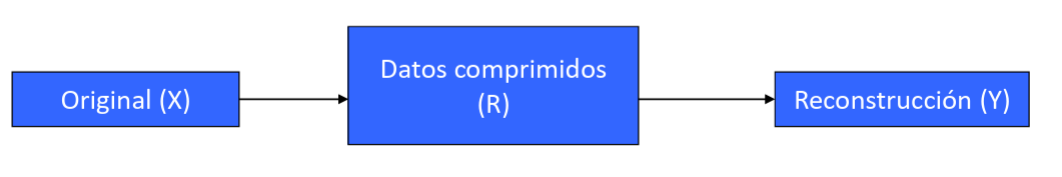
\includegraphics[width=0.85\linewidth]{resources/Coder_Decoder.png}
    \caption{Esquema de codificación y decodificación en un sistema de compresión.}
    \label{fig:coder-decoder}
\end{figure}

Un sistema de compresión consta de dos procesos: \textbf{codificación} y \textbf{decodificación}.

\begin{NotaBox}
Un sistema de compresión puede ser:
\begin{itemize}
    \item \textbf{Asimétrico}: el codificador es más complejo que el decodificador.
    \item \textbf{Simétrico}: el codificador y el decodificador tienen la misma complejidad.
    \item \textbf{Con pérdidas o irreversible}: aplicado a vídeo, audio, imagen.
    \item \textbf{Sin pérdidas o reversible}: aplicado a texto.
\end{itemize}
\end{NotaBox}

\subsection{Factores de diseño}

\begin{ChecklistBox}
Factores a considerar en el diseño de un codificador:
\begin{itemize}
    \item Retardo.
    \item Eficiencia (tasa de compresión).
    \item Complejidad.
    \item Calidad de la señal.
\end{itemize}
\end{ChecklistBox}

\begin{RecordatorioBox}
La mayoría de los estándares usan compresión con pérdidas, lo que permite alcanzar mayores tasas de compresión.
\end{RecordatorioBox}

\begin{figure}[!htbp]
    \centering
    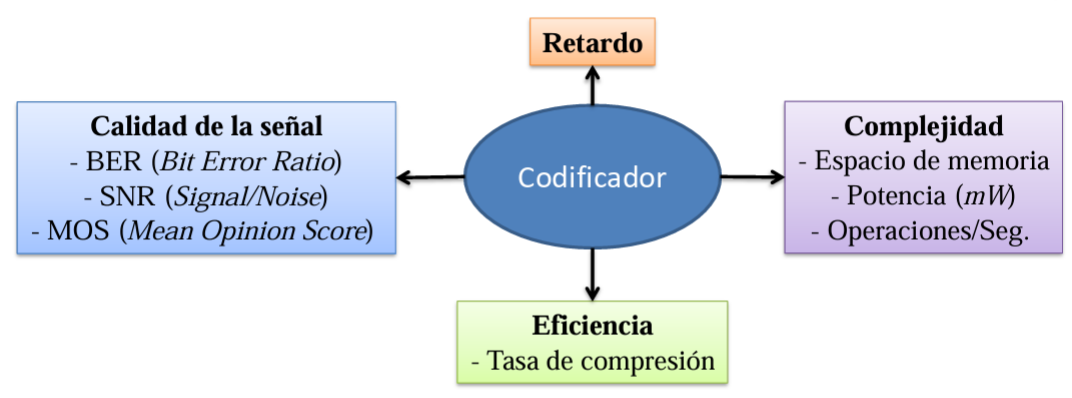
\includegraphics[width=0.85\linewidth]{resources/Coder_Metrics.png}
    \caption{Métricas típicas para evaluar un sistema de codificación.}
    \label{fig:coder-metrics}
\end{figure}

\section{Técnicas de compresión}

\subsection{Codificación entrópica}
Ejemplo: compresión \texttt{zip}.
Son independientes de las características del medio, por lo que se consideran universales.

\subsection{Codificación de fuente}
Codifica los datos basándose en las características del medio.
Suelen ser técnicas con pérdidas.
Permiten tasas de compresión elevadas.
Se aplican mediante codificadores de propósito específico.

\subsection{Codificación híbrida}
La mayoría de algoritmos pertenecen a este tipo.

\begin{ResumenBox}
Codificación entrópica es universal.
Codificación de fuente explota características del medio.
Codificación híbrida combina ambas.
\end{ResumenBox}

\begin{VocabBox}
\begin{itemize}
	\item \textbf{Compresión}: reducción del tamaño de los datos.
	\item \textbf{Codificación}: proceso de transformar los datos para reducir espacio.
	\item \textbf{Decodificación}: proceso de reconstrucción de los datos.
\end{itemize}
\end{VocabBox}

\subsection{Ejemplos}

\begin{figure}[!htbp]
	\centering
	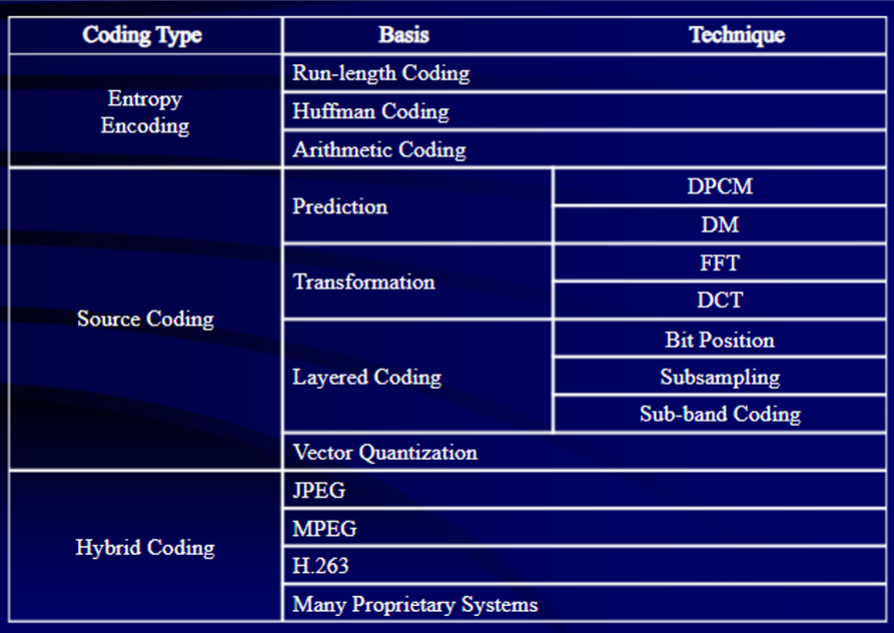
\includegraphics[width=0.8\linewidth]{resources/Compression_Types_Examples}
	\caption{Ejemplos de tipos de compresión: sin pérdidas, con pérdidas y mixtas.}
	\label{fig:compression-types-examples}
\end{figure}

\subsection{Compresión sin pérdidas}
\begin{itemize}
	\item \textbf{Técnicas estadísticas}
	\begin{itemize}
		\item \textbf{Codificación Huffman}:
		\item \textbf{Codificación aritmética}
	\end{itemize}
	\item \textbf{Técnicas basadas en diccionarios}
	\begin{itemize}
		\item \textbf{Lempel-Ziv-Welch (LZW)}:
	\end{itemize}
	\item \textbf{Técnicas predictivas}
	\begin{itemize}
		\item \textbf{Predicción y codificación del residuo}:
	\end{itemize}
\end{itemize}

\begin{NotaBox}
Los estándares suelen definir únicamente la parte de descompresión (decodificador).
\end{NotaBox}

\subsection{Compresión con pérdidas}

Se utiliza en ámbitos donde no es necesario reconstruir exactamente la señal original, como en:
\begin{itemize}
    \item Vídeos
    \item Audio
    \item Imágenes
\end{itemize}

\textbf{Técnicas:}
\begin{itemize}
    \item Cuantificación escalar
    \item Wavelets
    \item Transformación por bloques
\end{itemize}

\textbf{Estándares:}
\begin{itemize}
    \item JPEG
    \item JPEG 2000
    \item MPEG
\end{itemize}

\section{Conceptos Básicos}
\subsection{Calidad de un algoritmo de compresión}

Es necesario tener en cuenta:
\begin{itemize}
    \item Complejidad del algoritmo.
    \item Necesidad de memoria.
    \item Tiempo de ejecución.
    \item Cantidad de compresión.
    \item Grado de similitud entre la reconstrucción y los datos originales.
\end{itemize}

\subsection{Teoría de la información}

\begin{DefBox}
\textbf{Fuente:} par $(S, P)$

\begin{itemize}
    \item $S$ es un conjunto finito de mensajes denominado \textbf{alfabeto de la fuente}.
    \item $P : S \to [0,1]$ es una función de probabilidad que asigna a cada símbolo $s \in S$ su probabilidad de aparición $P(s)$.
    \item La probabilidad de un mensaje $s_1$ es $P(s_1)$.
\end{itemize}
\end{DefBox}

\begin{NotaBox}
Cuanto mayor sea la probabilidad de un mensaje, menor será su contenido de información.

Una fuente formada por mensajes de baja probabilidad aporta más información que una fuente compuesta por pocos mensajes de alta probabilidad.
\end{NotaBox}

\subsection{Cantidad de información}

La cantidad de información de un suceso $A$, con probabilidad de ocurrencia $P(A)$, se define como:

\[
I(A) = - \log_{2}\!\big(P(A)\big)
\]

La unidad de la información depende de la base del logaritmo:
\begin{itemize}
	\item Base 2: bits
	\item Base 10: Hartleys
	\item Base $e$: nats
\end{itemize}

Si 2 sucesos $A$ y $B$ son independientes, la cantidad de información conjunta es:
\[
I(A \cap B) = I(A) + I(B)
\]

\textbf{Ejemplo:}
Sea un experimento con dos sucesos independientes, cada uno con probabilidad $P(A) = \frac{1}{2}$.
La información asociada al suceso $A$ se calcula como:
\[
I(A) = -\log_2 P(A) = -\log_2 \left(\frac{1}{2}\right) = 1 \text{ bit.}
\]

\subsection*{Ejemplo: Cálculo de la información de una secuencia de mensajes}

Dada la secuencia de mensajes:
\[
1, 2, 3, 2, 3, 4, 5, 4, 5, 6, 7, 8, 9, 8, 9, 10
\]

La \textbf{fórmula de la información} se define como:
\[
I(A) = -\log_2 P(A)
\]

\begin{table}[h!]
\centering
\caption{Cálculo de la información por mensaje}
\begin{tabular}{cccc}
\toprule
\textbf{Mensaje} & \textbf{Apariciones} & \textbf{Probabilidad $P(A)$} & \textbf{Información $I(A)$ (bits)} \\
\midrule
1  & 1 & $\tfrac{1}{16}$ & 4 \\
2  & 2 & $\tfrac{1}{8}$  & 3 \\
3  & 2 & $\tfrac{1}{8}$  & 3 \\
4  & 2 & $\tfrac{1}{8}$  & 3 \\
5  & 2 & $\tfrac{1}{8}$  & 3 \\
6  & 1 & $\tfrac{1}{16}$ & 4 \\
7  & 1 & $\tfrac{1}{16}$ & 4 \\
8  & 2 & $\tfrac{1}{8}$  & 3 \\
9  & 2 & $\tfrac{1}{8}$  & 3 \\
10 & 1 & $\tfrac{1}{16}$ & 4 \\
\bottomrule
\end{tabular}
\end{table}

La información de un conjunto de mensajes es la suma de las informaciones individuales:
\[
I(\text{secuencia}) = 4 + 3 + 3 + 3 + 3 + 4 + 4 + 3 + 3 + 4 = 34 \text{ bits}
\]

\subsection{Entropía de una fuente}

Dada una fuente $(S, P)$, la \textbf{entropía} $H(S)$ se define como:
\[
H(S) = - \sum_{s \in S} P(s) \log_2 P(s)
\]

\begin{itemize}
	\item La entropía es la mínima longitud promedio de bits por símbolo necesaria para codificar la fuente sin pérdidas.
	\item El número medio de bits nunca será menor que la entropía.
	\item Si la probabilidad de todos los símbolos es igual, la entropía es máxima. Por ejemplo, si hay $N$ símbolos con la misma probabilidad, entonces $P(s) = \frac{1}{N}$ y:
	\[H(S) = \log_2 N\]
	\item Si un símbolo tiene probabilidad 1, la entropía es 0
	\item La entropía es la incertidubre que tengo de que me llegue un símbolo u otro.
\end{itemize}

\subsubsection*{Ejemplo: Entropía con probabilidades no equiprobables}
Para $S=\{A,B,C,D\}$ con $P(A)=\tfrac12$, $P(B)=\tfrac14$ y $P(C)=P(D)=\tfrac18$:
\[
\begin{aligned}
H(S) &= -\Big(\tfrac12\log_2\tfrac12 + \tfrac14\log_2\tfrac14 + \tfrac18\log_2\tfrac18 + \tfrac18\log_2\tfrac18\Big) \\
	&= \tfrac12\cdot 1 + \tfrac14\cdot 2 + \tfrac18\cdot 3 + \tfrac18\cdot 3 \\
	&= 1{,}75 \text{ bits.}
\end{aligned}
\]

\begin{NotaBox}
Si los cuatro símbolos fueran equiprobables ($P(s)=\tfrac14$), entonces
$H_{\text{eq}}=\log_2 4 = 2$ bits. Como $1{,}75<2$, concentrar probabilidad en
algunos símbolos reduce la entropía.
\end{NotaBox}

Cuando hay un simbolo con más probabilidad que los demás, la entropía disminuye. Tenemos menos incertidubre sobre qué símbolo va a llegar.
\subsection{Códigos}

\textbf{Alfabeto:} conjunto de letras o símbolos utilizados para formar mensajes.

\medskip

\textbf{Código:} es un conjunto finito y no vacío de cadenas construidas a partir de un alfabeto.
Cada cadena individual dentro del código se denomina \emph{palabra clave} o \emph{palabra código}.

\medskip

En términos formales, un \textbf{código} puede considerarse como una \emph{aplicación} o \emph{mapeo} entre dos conjuntos:
\begin{itemize}
    \item Un conjunto de símbolos denominado \textbf{alfabeto fuente}.
    \item Otro conjunto de símbolos denominado \textbf{alfabeto código}.
\end{itemize}

De esta forma, cada símbolo del alfabeto fuente se representa mediante una palabra código en el alfabeto código.

\textbf{Esquema de codificación:}

\[
f: S \rightarrow C^{+}
\]

donde:
\begin{itemize}
    \item $S$ representa el \textbf{alfabeto fuente}.
    \item $C$ representa el \textbf{alfabeto código}.
    \item $C^{+}$ denota el conjunto de todas las \textbf{cadenas no vacías} formadas a partir de los símbolos de $C$.
\end{itemize}

El esquema de codificación se define como una \textbf{función inyectiva}, es decir, a cada símbolo del alfabeto fuente le corresponde una única palabra código, y no existen dos símbolos distintos que tengan la misma representación.

\textbf{Código unívocamente descifrable:}
Un código es \emph{unívocamente descifrable} si, para cualquier secuencia de símbolos perteneciente al alfabeto código,
existe como máximo una única secuencia de palabras código que pueda generar dicha secuencia.

En otras palabras, la función de esquema de codificación es \textbf{reversible},
ya que permite recuperar de manera única el mensaje original a partir de la secuencia codificada.

\textbf{Código instantáneo:}
Un código es \emph{instantáneo} si cada palabra código puede ser identificada y decodificada a medida que se recibe,
leyendo la secuencia de izquierda a derecha, sin necesidad de conocer los símbolos que la siguen.

\textbf{Código prefijo:}
Un código es \emph{prefijo} si ninguna de sus palabras código es prefijo de otra.

\medskip

\textbf{Ejemplo:}
El conjunto $\{0,\, 10,\, 110,\, 111\}$ es un código prefijo,
mientras que $\{0,\, 01,\, 011\}$ no lo es, ya que \texttt{0} es prefijo de las demás.

\begin{NotaBox}
Relaciones clave entre clases de códigos:
\begin{itemize}
	\item \textbf{Prefijo} $\Rightarrow$ \textbf{instantáneo}.
	\item \textbf{Prefijo} (e instantáneo) $\Rightarrow$ \textbf{unívocamente descifrable}.
	\item Existen códigos \textbf{unívocamente descifrables} que no son instantáneos (ni prefijo), p. ej. $\{0,01\}$.
\end{itemize}
\end{NotaBox}

\begin{NotaBox}
Un código se denomina óptimo cuando es instantaneo y únivocamente descifrable.
\end{NotaBox}

\section{Medidas de Compresión}

A continuación se presentan las principales medidas empleadas para evaluar la eficiencia de un algoritmo de compresión.

\subsection*{Definiciones}

\begin{itemize}
    \item $o$: Longitud del archivo original (en bytes).
    \item $c$: Longitud del archivo comprimido (en bytes).
\end{itemize}

\subsection*{Fórmulas}

\paragraph{Longitud media por símbolo (LMS):}
\begin{equation}
    \mathrm{LMS} = \frac{c \times 8}{o} \quad [\text{bits/símbolo}]
\end{equation}

Cuando se trabaja con imágenes, esta métrica se expresa como \textbf{bits por píxel (bpp)}.

\paragraph{Factor o razón de compresión (FC):}
\begin{equation}
    \mathrm{FC} = \frac{o}{c}
\end{equation}
Por ejemplo, un valor de $\mathrm{FC} = 3$ indica una compresión de $3\!:\!1$.

\paragraph{Tamaño comprimido relativo (TCR):}
\begin{equation}
    \mathrm{TCR} = \frac{c}{o}
\end{equation}
Por ejemplo, un valor de $\mathrm{TCR} = 0.33$.

\paragraph{Compresión relativa (CR):}
\begin{equation}
    \mathrm{CR} = \frac{o - c}{o} = 1 - \mathrm{TCR}
\end{equation}
Por ejemplo, un valor de $\mathrm{CR} = 0.66$.

\section{Medidas de Error}

Las medidas de error permiten cuantificar la diferencia entre una señal original y su versión reconstruida o aproximada después de un proceso de compresión. A continuación, se presentan las métricas más utilizadas.

\subsection*{Error cuadrático medio (MSE)}

El \textbf{Error Cuadrático Medio} (\textit{Mean Squared Error}, MSE) mide la diferencia promedio al cuadrado entre los valores originales y los valores reconstruidos. Se define como:

\begin{equation}
    \mathrm{MSE} = \frac{1}{N} \sum_{i=1}^{N} (x_i - y_i)^2
\end{equation}

donde:
\begin{itemize}
    \item $x_i$ es el valor original,
    \item $y_i$ es el valor reconstruido o aproximado,
    \item $N$ es el número total de muestras o elementos comparados.
\end{itemize}

\paragraph{MSE para imágenes.}
Sean $I$ e $I'$ dos imágenes de tamaño $n \times m$, donde $I'$ es una aproximación de $I$. El MSE entre ambas imágenes se calcula como:

\begin{equation}
    \mathrm{MSE}(I, I') = \frac{1}{n \, m} \sum_{i=0}^{n-1} \sum_{j=0}^{m-1} \bigl[ I(i,j) - I'(i,j) \bigr]^2
\end{equation}

\subsection*{Relación pico señal a ruido (PSNR)}

El \textbf{Peak Signal-to-Noise Ratio} (PSNR) se emplea comúnmente para evaluar la calidad de imágenes o vídeos comprimidos. Se define en función del MSE como:

\begin{equation}
    \mathrm{PSNR} = 10 \, \log_{10} \left( \frac{L^2}{\mathrm{MSE}} \right)
\end{equation}

donde $L$ representa el valor máximo posible de un píxel (por ejemplo, $L = 255$ para imágenes de 8 bits por canal).

La unidad de medida del PSNR es el \textbf{decibelio (dB)}. Valores más altos de PSNR indican una mejor calidad de reconstrucción.

\section{Proceso de Compresión}

Se divide en dos fases. Modelización y codificación.
\begin{figure}[!htbp]
	\centering
	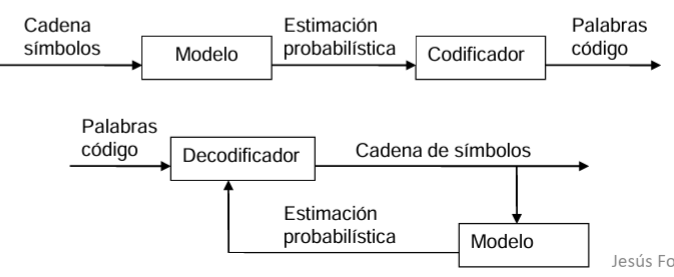
\includegraphics[width=0.85\linewidth]{resources/Compression_Process.png}
	\caption{Fases del proceso de compresión: modelización y codificación.}
	\label{fig:compression-process}
\end{figure}

El modelo puede abstraerse de la fuente, puede generalizar detalles específicos.

El modelo puede ser deterministico, es decir, mismo comportamiento en el descodificador como en el codificador.

Un modelo realiza una estimación de la probabilidad de los símbolos.

\subsection{Modelo no adaptativo}

Probabilidad de cada simbolo predefinida. Es una información que tanto el codificador como el decodificador conocen de antemano.
Simple y fácil de implementar, pero no se adapta a cambios en la fuente.

\subsection{Modelo semi-adaptativo}

Realiza una primera lectura de los datos a comprimir para así asignar las probabilidades de los símbolos.

Se necesita tener el mensaje completo antes de codificar, introduce overhead, requiere enviar la codificación de las probabilidades al decodificador.

\subsection{Modelo Adaptativo}
Su funcionamiento permite analizar la distribución de los símbolos a medida que se van procesando. No requiere una pasada previa por los datos ni enviar información adicional al decodificador.

Comforme se vayan procesando los símbolos, se van actualizando las probabilidades. Sirve para streaming de datos.

\subsection{Codificadores estadísticos}
Especialmente útiles en la compresión de imágenes
Se basan en asignar palabras codigo a partir de las estimaciones de aparación de los símbolos. Dos tipos
codigos de prefijo y codigos aritmeticos.

\end{document}
